\documentclass[journal,12pt,twocolumn]{IEEEtran}
%
\usepackage{setspace}
\usepackage{gensymb}
\usepackage{xcolor}
\usepackage{caption}
%\usepackage{subcaption}
%\doublespacing
\singlespacing

%\usepackage{graphicx}
%\usepackage{amssymb}
%\usepackage{relsize}
\usepackage[cmex10]{amsmath}
\usepackage{mathtools}
%\usepackage{amsthm}
%\interdisplaylinepenalty=2500
%\savesymbol{iint}
%\usepackage{txfonts}
%\restoresymbol{TXF}{iint}
%\usepackage{wasysym}
\usepackage{amsthm}
\usepackage{mathrsfs}
\usepackage{txfonts}
\usepackage{stfloats}
\usepackage{cite}
\usepackage{cases}
\usepackage{subfig}
%\usepackage{xtab}
\usepackage{longtable}
\usepackage{multirow}
%\usepackage{algorithm}
%\usepackage{algpseudocode}
\usepackage{enumitem}
\usepackage{mathtools}
\usepackage{iithtlc}
%\usepackage[framemethod=tikz]{mdframed}
\usepackage{listings}


%\usepackage{stmaryrd}


%\usepackage{wasysym}
%\newcounter{MYtempeqncnt}
\DeclareMathOperator*{\Res}{Res}
%\renewcommand{\baselinestretch}{2}
\renewcommand\thesection{\arabic{section}}
\renewcommand\thesubsection{\thesection.\arabic{subsection}}
\renewcommand\thesubsubsection{\thesubsection.\arabic{subsubsection}}

\renewcommand\thesectiondis{\arabic{section}}
\renewcommand\thesubsectiondis{\thesectiondis.\arabic{subsection}}
\renewcommand\thesubsubsectiondis{\thesubsectiondis.\arabic{subsubsection}}

% correct bad hyphenation here
\hyphenation{op-tical net-works semi-conduc-tor}

\lstset{
language=Python,
frame=single, 
breaklines=true
}

%\lstset{
	%%basicstyle=\small\ttfamily\bfseries,
	%%numberstyle=\small\ttfamily,
	%language=Octave,
	%backgroundcolor=\color{white},
	%%frame=single,
	%%keywordstyle=\bfseries,
	%%breaklines=true,
	%%showstringspaces=false,
	%%xleftmargin=-10mm,
	%%aboveskip=-1mm,
	%%belowskip=0mm
%}

%\surroundwithmdframed[width=\columnwidth]{lstlisting}


\begin{document}
%

\theoremstyle{definition}
\newtheorem{theorem}{Theorem}[section]
\newtheorem{problem}{Problem}
\newtheorem{proposition}{Proposition}[section]
\newtheorem{lemma}{Lemma}[section]
\newtheorem{corollary}[theorem]{Corollary}
\newtheorem{example}{Example}[section]
\newtheorem{definition}{Definition}[section]
%\newtheorem{algorithm}{Algorithm}[section]
%\newtheorem{cor}{Corollary}
\newcommand{\BEQA}{\begin{eqnarray}}
\newcommand{\EEQA}{\end{eqnarray}}
\newcommand{\define}{\stackrel{\triangle}{=}}

\bibliographystyle{IEEEtran}
%\bibliographystyle{ieeetr}

\providecommand{\nCr}[2]{\,^{#1}C_{#2}} % nCr
\providecommand{\nPr}[2]{\,^{#1}P_{#2}} % nPr
\providecommand{\mbf}{\mathbf}
\providecommand{\pr}[1]{\ensuremath{\Pr\left(#1\right)}}
\providecommand{\qfunc}[1]{\ensuremath{Q\left(#1\right)}}
\providecommand{\sbrak}[1]{\ensuremath{{}\left[#1\right]}}
\providecommand{\lsbrak}[1]{\ensuremath{{}\left[#1\right.}}
\providecommand{\rsbrak}[1]{\ensuremath{{}\left.#1\right]}}
\providecommand{\brak}[1]{\ensuremath{\left(#1\right)}}
\providecommand{\lbrak}[1]{\ensuremath{\left(#1\right.}}
\providecommand{\rbrak}[1]{\ensuremath{\left.#1\right)}}
\providecommand{\cbrak}[1]{\ensuremath{\left\{#1\right\}}}
\providecommand{\lcbrak}[1]{\ensuremath{\left\{#1\right.}}
\providecommand{\rcbrak}[1]{\ensuremath{\left.#1\right\}}}
\theoremstyle{remark}
\newtheorem{rem}{Remark}
\newcommand{\sgn}{\mathop{\mathrm{sgn}}}
\providecommand{\abs}[1]{\left\vert#1\right\vert}
\providecommand{\res}[1]{\Res\displaylimits_{#1}} 
\providecommand{\norm}[1]{\lVert#1\rVert}
\providecommand{\mtx}[1]{\mathbf{#1}}
\providecommand{\mean}[1]{E\left[ #1 \right]}
\providecommand{\fourier}{\overset{\mathcal{F}}{ \rightleftharpoons}}
%\providecommand{\hilbert}{\overset{\mathcal{H}}{ \rightleftharpoons}}
\providecommand{\system}{\overset{\mathcal{H}}{ \longleftrightarrow}}
	%\newcommand{\solution}[2]{\textbf{Solution:}{#1}}
\newcommand{\solution}{\noindent \textbf{Solution: }}
\providecommand{\dec}[2]{\ensuremath{\overset{#1}{\underset{#2}{\gtrless}}}}
%\numberwithin{equation}{subsection}
\numberwithin{equation}{problem}
%\numberwithin{problem}{subsection}
%\numberwithin{definition}{subsection}
\makeatletter
\@addtoreset{figure}{problem}
\makeatother

\let\StandardTheFigure\thefigure
%\renewcommand{\thefigure}{\theproblem.\arabic{figure}}
\renewcommand{\thefigure}{\theproblem}


%\numberwithin{figure}{subsection}

\def\putbox#1#2#3{\makebox[0in][l]{\makebox[#1][l]{}\raisebox{\baselineskip}[0in][0in]{\raisebox{#2}[0in][0in]{#3}}}}
     \def\rightbox#1{\makebox[0in][r]{#1}}
     \def\centbox#1{\makebox[0in]{#1}}
     \def\topbox#1{\raisebox{-\baselineskip}[0in][0in]{#1}}
     \def\midbox#1{\raisebox{-0.5\baselineskip}[0in][0in]{#1}}

\vspace{3cm}

\title{ 
\logo{
Python for Signals and Systems 
}
%	\logo{Octave for Math Computing }
}
%\title{
%	\logo{Matrix Analysis through Octave}{\begin{center}\includegraphics[scale=.24]{tlc}\end{center}}{}{HAMDSP}
%}


% paper title
% can use linebreaks \\ within to get better formatting as desired
%\title{Matrix Analysis through Octave}
%
%
% author names and IEEE memberships
% note positions of commas and nonbreaking spaces ( ~ ) LaTeX will not break
% a structure at a ~ so this keeps an author's name from being broken across
% two lines.
% use \thanks{} to gain access to the first footnote area
% a separate \thanks must be used for each paragraph as LaTeX2e's \thanks
% was not built to handle multiple paragraphs
%

\author{Prashant Kumar Aleshwaram$^{\dagger}$, Mohammed Zafar Ali Khan$^{*}$ and G V V Sharma$^{*}$ %<-this  stops a space
\thanks{*The authors are with the Department
of Electrical Engineering, Indian Institute of Technology, Hyderabad
502285 India e-mail:  \{zafar,gadepall\}@iith.ac.in.$\dagger$ The author is an intern with the Teaching Learning Centre, IIT Hyderabad email: akumar10@student.nitw.ac.in. All content in the manuscript is released under GNU GPL.  Free to use for anything. }% <-this % stops a space
%\thanks{J. Doe and J. Doe are with Anonymous University.}% <-this % stops a space
%\thanks{Manuscript received April 19, 2005; revised January 11, 2007.}}
}
% note the % following the last \IEEEmembership and also \thanks - 
% these prevent an unwanted space from occurring between the last author name
% and the end of the author line. i.e., if you had this:
% 
% \author{....lastname \thanks{...} \thanks{...} }
%                     ^------------^------------^----Do not want these spaces!
%
% a space would be appended to the last name and could cause every name on that
% line to be shifted left slightly. This is one of those "LaTeX things". For
% instance, "\textbf{A} \textbf{B}" will typeset as "A B" not "AB". To get
% "AB" then you have to do: "\textbf{A}\textbf{B}"
% \thanks is no different in this regard, so shield the last } of each \thanks
% that ends a line with a % and do not let a space in before the next \thanks.
% Spaces after \IEEEmembership other than the last one are OK (and needed) as
% you are supposed to have spaces between the names. For what it is worth,
% this is a minor point as most people would not even notice if the said evil
% space somehow managed to creep in.



% The paper headers
%\markboth{Journal of \LaTeX\ Class Files,~Vol.~6, No.~1, January~2007}%
%{Shell \MakeLowercase{\textit{et al.}}: Bare Demo of IEEEtran.cls for Journals}
% The only time the second header will appear is for the odd numbered pages
% after the title page when using the twoside option.
% 
% *** Note that you probably will NOT want to include the author's ***
% *** name in the headers of peer review papers.                   ***
% You can use \ifCLASSOPTIONpeerreview for conditional compilation here if
% you desire.




% If you want to put a publisher's ID mark on the page you can do it like
% this:
%\IEEEpubid{0000--0000/00\$00.00~\copyright~2007 IEEE}
% Remember, if you use this you must call \IEEEpubidadjcol in the second
% column for its text to clear the IEEEpubid mark.



% make the title area
\maketitle

%\newpage

%\tableofcontents


%\begin{abstract}
%%\boldmath
%In this letter, an algorithm for evaluating the exact analytical bit error rate  (BER)  for the piecewise linear (PL) combiner for  multiple relays is presented. Previous results were available only for upto three relays. The algorithm is unique in the sense that  the actual mathematical expressions, that are prohibitively large, need not be explicitly obtained. The diversity gain due to multiple relays is shown through plots of the analytical BER, well supported by simulations. 
%
%\end{abstract}
% IEEEtran.cls defaults to using nonbold math in the Abstract.
% This preserves the distinction between vectors and scalars. However,
% if the journal you are submitting to favors bold math in the abstract,
% then you can use LaTeX's standard command \boldmath at the very start
% of the abstract to achieve this. Many IEEE journals frown on math
% in the abstract anyway.

% Note that keywords are not normally used for peerreview papers.
%\begin{IEEEkeywords}
%Cooperative diversity, decode and forward, piecewise linear
%\end{IEEEkeywords}



% For peer review papers, you can put extra information on the cover
% page as needed:
% \ifCLASSOPTIONpeerreview
% \begin{center} \bfseries EDICS Category: 3-BBND \end{center}
% \fi
%
% For peerreview papers, this IEEEtran command inserts a page break and
% creates the second title. It will be ignored for other modes.
\IEEEpeerreviewmaketitle

\bigskip

\begin{abstract}
This manual provides an introduction to signals and systems through simple python scripts.   
\end{abstract}


Problems \ref{prob1.1}-\ref{prob1.end} are related.
\begin{problem}
\label{prob1.1}
Let
\begin{equation}
x(n) = \cbrak{\underset{\uparrow}{0},2,3,1}
\end{equation}
Sketch $x(n)$
\end{problem}
\solution The following code yields Fig. \ref{fig_3a}.
\lstinputlisting{./codes/3a.py}
\begin{figure}[!h]
\begin{center}
\includegraphics[width=\columnwidth]{./figs/3a}
\end{center}
\captionof{figure}{}
\label{fig_3a}	
\end{figure}
%
\begin{problem}
Is $x(n)$
\begin{enumerate}
\item An energy signal?
\item A power signal?
\item A causal signal?
\item A periodic signal?
\end{enumerate}
\end{problem}
%
\begin{problem}
Sketch $3x(n)$.
\end{problem}
\solution The following code yields Fig. \ref{fig_3b}.
\lstinputlisting{./codes/3b.py}
\begin{figure}[!h]
\begin{center}
\includegraphics[width=\columnwidth]{./figs/3b}
\end{center}
\captionof{figure}{}
\label{fig_3b}	
\end{figure}
%
\begin{problem}
Sketch $x(n-2)$.
\end{problem}
\solution The following code yields Fig. \ref{fig_3c}.
\lstinputlisting{./codes/3c.py}
\begin{figure}[!h]
\begin{center}
\includegraphics[width=\columnwidth]{./figs/3c}
\end{center}
\captionof{figure}{}
\label{fig_3c}	
\end{figure}
%
\begin{problem}
\label{prob1.end}
Sketch $x(3-n)$.
\end{problem}
\solution The following code yields Fig. \ref{fig_3d}.
\lstinputlisting{./codes/3d.py}
\begin{figure}[!h]
\begin{center}
\includegraphics[width=\columnwidth]{./figs/3d}
\end{center}
\captionof{figure}{}
\label{fig_3d}	
\end{figure}
%
\begin{problem}
Sketch 
\begin{equation}
x(t) = 
\begin{cases}
4 - \abs{t} & 1 \leq \abs{t} \leq 4 \\
2 + \abs{t} & \abs{t} < 1
\end{cases}
\end{equation}
%
and find out if its even or odd.
\end{problem}
\solution The following code yields Fig. \ref{fig_4a}. As we can see, $x(t)=x(-t)$ and the function is even.
\lstinputlisting{./codes/4a.py}
\begin{figure}[!h]
\begin{center}
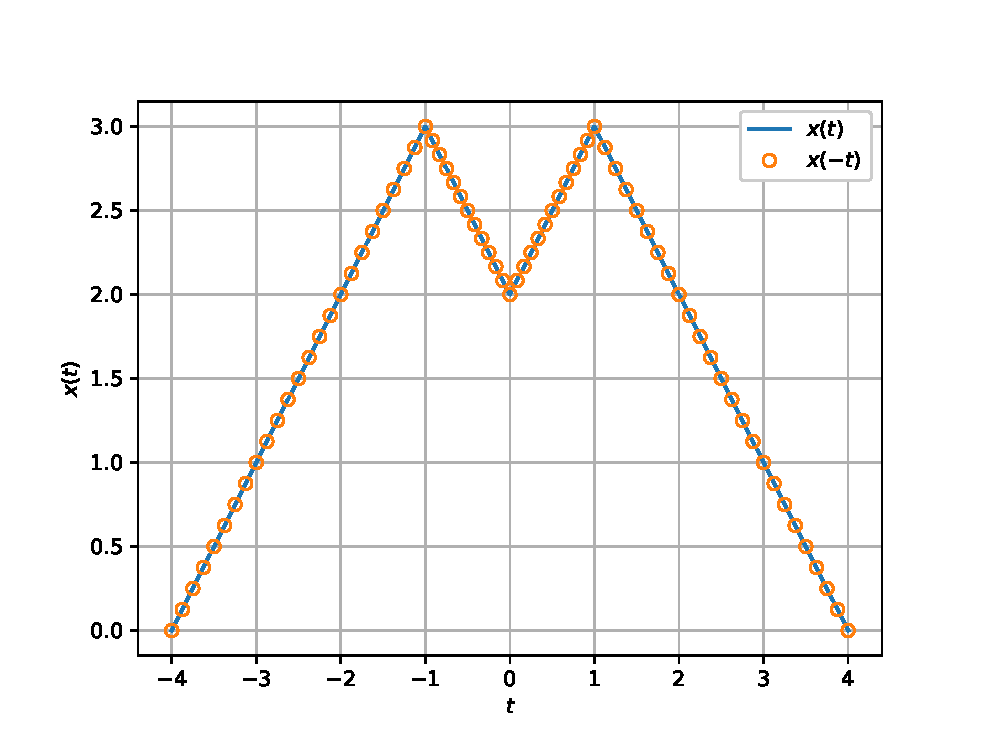
\includegraphics[width=\columnwidth]{./figs/4a}
\end{center}
\captionof{figure}{}
\label{fig_4a}	
\end{figure}
%

\begin{problem}
Sketch 
\begin{equation}
x(t) = 
\begin{cases}
t + 4 & -4 \leq t \leq -1 \\
-5t-2 & -1 < t < 0 \\
\frac{2}{3}\brak{t-3} & 0 \leq t \leq 3 \\
0 & \text{ otherwise }
\end{cases}
\end{equation}
%
and find out if its even or odd.
\end{problem}
\solution The following code yields Fig. \ref{fig_4b}. As we can see, the function is neither even nor odd.
\lstinputlisting{./codes/4b.py}
\begin{figure}[!h]
\begin{center}
\includegraphics[width=\columnwidth]{./figs/4b}
\end{center}
\captionof{figure}{}
\label{fig_4b}	
\end{figure}
%
\begin{problem}
Sketch 
\begin{equation}
x(t) = 
\begin{cases}
3\brak{t + 4} & -4 \leq t \leq -3 \\
-5t-12 & -3 < t < -2 \\
3t+4 & -2 \leq t \leq -1 \\
-t & -1 < t < 1 \\
3t-4 & 1 \le t \le 2 \\
-5t+12 & 2 < t < 3 \\
3\brak{t-4} & 3 \le t \le 4 \\
0 & \text{ otherwise }
\end{cases}
\end{equation}
%
and find out if its even or odd.
\end{problem}
\solution The following code yields Fig. \ref{fig_4c}. As we can see, $x(t)= -x(-t)$ and the function is odd.
\lstinputlisting{./codes/4c.py}
\begin{figure}[!h]
\begin{center}
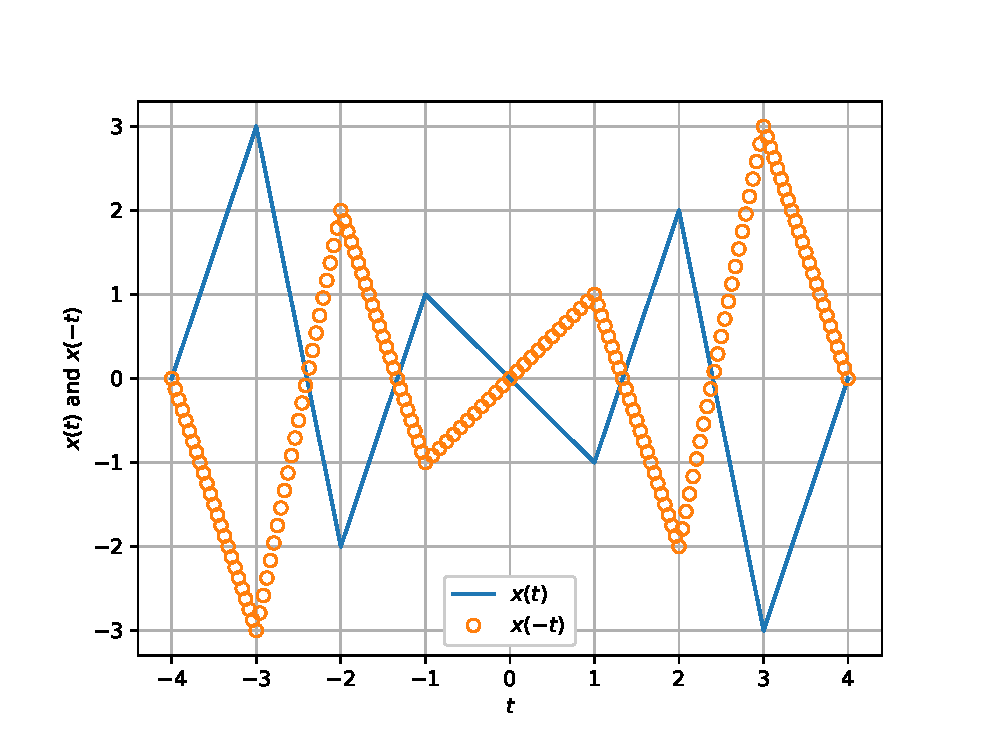
\includegraphics[width=\columnwidth]{./figs/4c}
\end{center}
\captionof{figure}{}
\label{fig_4c}	
\end{figure}
%
Problems \ref{prob2.1}-\ref{prob2.end} are related.
%
\begin{problem}
\label{prob2.1}
Sketch 
%
\begin{equation}
x(t) = 
\begin{cases}
t + 4 & -4 \le t \le -2 \\
t-4 & 2 \le t \le  4 \\
0 & \text{ otherwise }
\end{cases}
\end{equation}
%
\end{problem}
\solution The following code yields Fig. \ref{fig_8}
\lstinputlisting{./codes/8.py}
\begin{figure}[!h]
\begin{center}
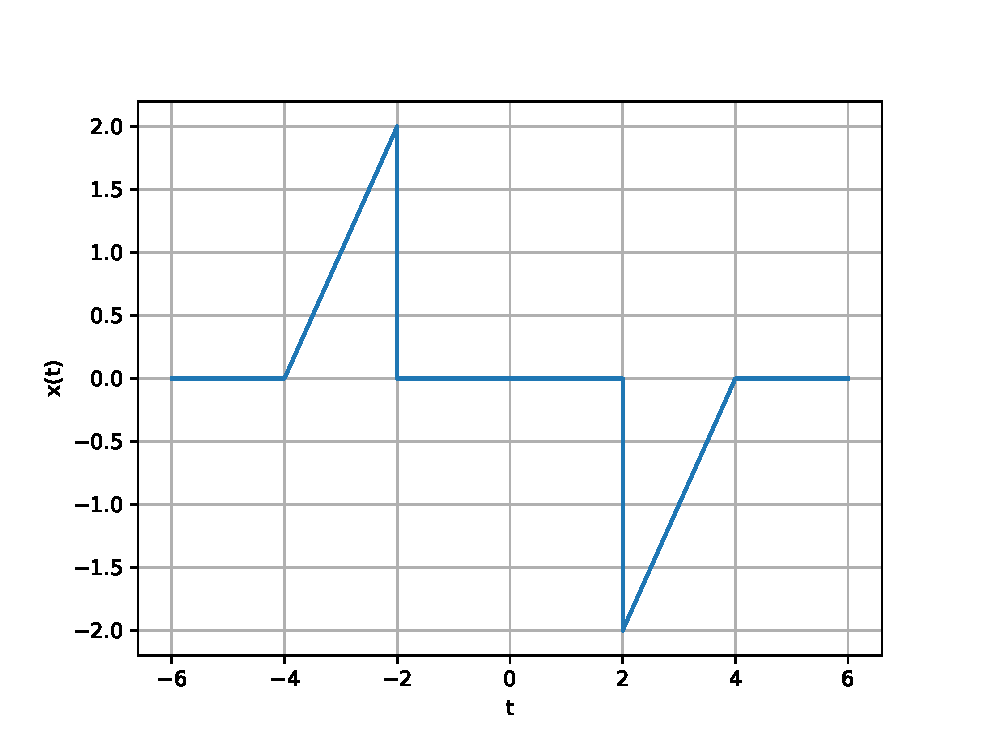
\includegraphics[width=\columnwidth]{./figs/8}
\end{center}
\captionof{figure}{}
\label{fig_8}	
\end{figure}
%
\begin{problem}
Sketch  $x(t+1)$
\end{problem}
%
\solution The following code yields Fig. \ref{fig_8a}
\lstinputlisting{./codes/8a.py}
\begin{figure}[!h]
\begin{center}
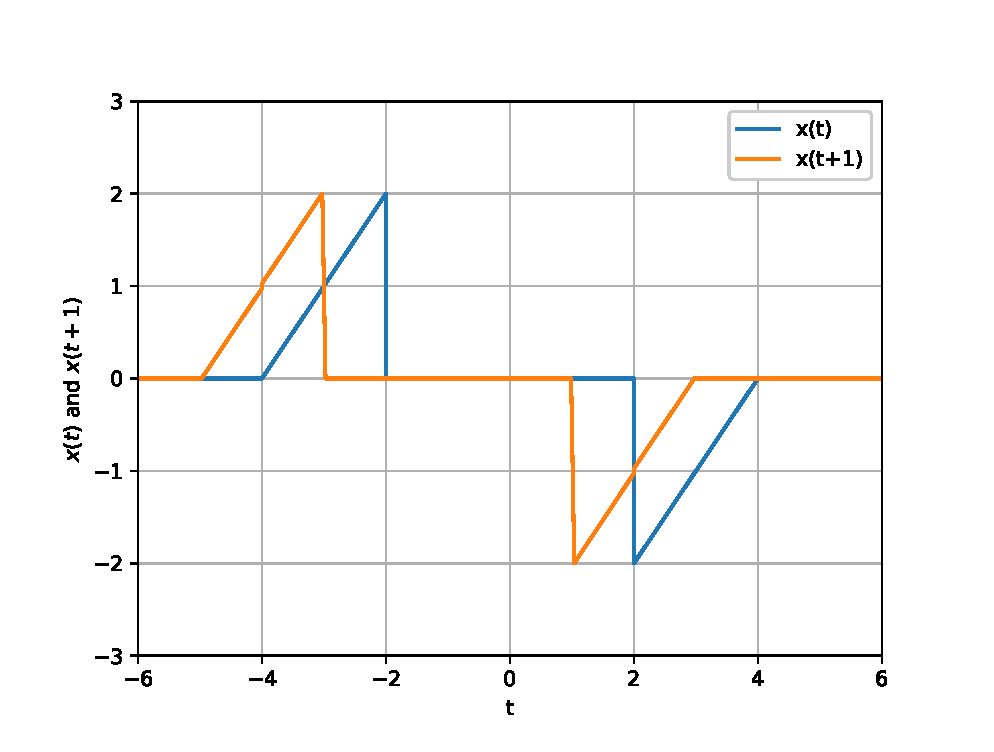
\includegraphics[width=\columnwidth]{./figs/8a}
\end{center}
\captionof{figure}{}
\label{fig_8a}	
\end{figure}
%
\begin{problem}
Sketch $5x\brak{\frac{t}{3}}$
\end{problem}
\begin{problem}
Sketch  $2x(t-2)$
\end{problem}
%
%
\begin{problem}
\label{prob2.end}
Sketch  $x(t)-x(-t)$.
\end{problem}
%
Problems \ref{prob3.1}-\ref{prob3.end} are related.
\begin{problem}
\label{prob3.1}
Let $x(t) = e^{-t}$  and $y(t) = x(t)u(t)$. Sketch $x(t)$ and $y(t)$.
\end{problem}
%
\begin{problem}
Sketch $x_1(t) = x(t-2)$ and $y_1(t)$, where $y_1(t)$ is the output when $x_1(t)$ is the input to the system.
\end{problem}
%
\begin{problem}
\label{prob3.end}
Sketch $y(t-2)$ and $y_1(t)$ in the same graph.  Is the system time invariant?
\end{problem}
%
Problems \ref{prob4.1}-\ref{prob4.end} are related.
\begin{problem}
\label{prob4.1}
If $x(t) = u(t)$, sketch
\begin{equation}
y(t) = \sum_{m=-1}^{2}mx(t-m)
\end{equation}
%
\end{problem}
%
\begin{problem}
\label{prob4.end}
Sketch $h(t)$ for the previous problem.  Is the system causal?
\end{problem}
%
Problems \ref{prob5.1}-\ref{prob5.end} are related.
\begin{problem}
\label{prob5.1}
Sketch
\begin{equation}
x(k) = \cbrak{-1,-1,-\underset{\uparrow}{1},1,-1,1,1,1}
\end{equation}
and
\begin{equation}
h(k) = \cbrak{\underset{\uparrow}{0},-1,1}
\end{equation}
\end{problem}
%
\begin{problem}
Sketch $h(-k)$ and $x(k)h(n-k)$ for $n = -2,-1, \dots,7 $.
\end{problem}
%
\begin{problem}
Sketch  $y(n) = \sum_{k}x(k)h(n-k)$ for $n = -2,-1, \dots,7 $.
\end{problem}
%
\begin{problem}
Run the following code and compare with the result of the previous problem.
\lstinputlisting{./codes/15.py}
\end{problem}
%
\begin{problem}
\label{prob5.end}
Sketch $h(n)*h(-n)$.
\end{problem}
%\solution The following code yields Fig. \ref{fig_8b}
%\lstinputlisting{./codes/8b.py}
%\begin{figure}[!h]
%\begin{center}
%\includegraphics[width=\columnwidth]{./figs/8b}
%\end{center}
%\captionof{figure}{}
%\label{fig_8b}	
%\end{figure}


%\begin{problem}
%Download the aud1.mp3 file from the following link
%\end{problem}
%%
%\begin{problem}
%Convert the aud1.mp3 file to aud1.wav file
%\end{problem}

%\solution
%\input{./problems/ee16b1001.tex}
%\lstinputlisting{./codes/ee16b1001.py}
%%
%\begin{problem}
%If $P = 
%\begin{pmatrix}
%\frac{\sqrt{3}}{2} & \frac{1}{2} \\
%-\frac{1}{2} & \frac{\sqrt{3}}{2}
%\end{pmatrix}, A = 
%\begin{pmatrix}
%1 & 1 \\
%0 & 1
%\end{pmatrix}
%$ and $Q = P A P^{T}$, find $P^{T}Q^{2015} P$.
%\end{problem}
%\solution
%\input{./problems/ee16b1002.tex}
%\lstinputlisting{./codes/ee16b1002.py}
%\begin{problem}
%Evaluate $\sum_{r=1}^{15}r^2 \frac{\binom{15}{r}}{\binom{15}{r-1}}$.
%\end{problem}
%\solution
%\input{./problems/ee16b1003.tex}
%\lstinputlisting{./codes/ee16b1003.py}
%\begin{problem}
%If 
%\begin{align}
%\label{prob_four}
%\lim_{x \rightarrow \infty} \brak{1 + \frac{a}{x} - \frac{4}{x^2}}^{2x} = e^3,
%\end{align}
% find $a$.
%\end{problem}
%\solution 
%\input{./problems/ee16b1004.tex}
%The following octave code yields Fig. \ref{fig_4} verifying the above result.
%\lstinputlisting{./codes/ee16b1004.py}
%\begin{figure}[!ht]
%\begin{center}
%\includegraphics[width=\columnwidth]{./figs/ee16b1004}
%\end{center}
%\captionof{figure}{LHS and RHS in \eqref{prob_four}}
%\label{fig_4}	
%\end{figure}
%\begin{problem}
%The function
%%
%\begin{equation}
%f(x)=
%\begin{cases}
%-x & x < 1 \\
%a + \cos^{-1}\brak{x + b} & 1 \leq x \leq 2
%\end{cases}
%\end{equation}
%%
%is known to be differentiable at $x=1$.  What is the value of $\frac{a}{b}$?
%\end{problem}
%\solution
%\input{./problems/ee16b1005.tex}
%The following octave code yields Fig. \ref{fig_5} verifying the above result.
%\lstinputlisting{./codes/ee16b1005.py}
%\begin{figure}[!ht]
%\begin{center}
%\includegraphics[width=\columnwidth]{./figs/ee16b1005}
%\end{center}
%\captionof{figure}{Substituting the values of $a$ and $b$ in $f(x)$, the graph is smooth at $x=1$. So $f(x)$ is differentiable $x=1$.}
%\label{fig_5}	
%\end{figure}
%%
%\begin{problem}
%The tangent at point $P$, for the curve $x = 4t^2+3, y = 8t^3-1$, with parameter $t \in \mathbf{R}$, meets the curve again at $Q$.  Find the coordinates of $Q$.
%\end{problem}
%\solution 	
%\input{./problems/ee16b1006.tex}
%The following code generates the plot in Fig. \ref{fig_6} for this problem. 
%\lstinputlisting{./codes/ee16b1006.py}
%\begin{figure}[!ht]
%\begin{center}
%\includegraphics[width=\columnwidth]{./figs/ee16b1006}
%\end{center}
%\captionof{figure}{The tangent at $P$ meets the curve again at $Q$.}
%\label{fig_6}	
%\end{figure}
%%
%\begin{problem}
%Find the minimum distance of a point on the curve $y = x^2 -4$ from the origin.
%\end{problem}
%\solution
%\input{./problems/ee16b1007.tex}
%The following code yields Figs. \ref{fig_7a} and \ref{fig_7b} explaining the solution.
%\lstinputlisting{./codes/ee16b1007.py}
%\renewcommand{\thefigure}{\theproblem.\arabic{figure}}
%
%\begin{figure}[!h]
%\begin{center}
%\includegraphics[width=\columnwidth]{./figs/ee16b1007a}
%\end{center}
%\captionof{figure}{The minimum distance is $\frac{\sqrt{17}}{2}$ for $k = -\frac{1}{2}$}
%\label{fig_7a}	
%\end{figure}
%%
%\begin{figure}[!h]
%\begin{center}
%\includegraphics[width=\columnwidth]{./figs/ee16b1007b}
%\end{center}
%\captionof{figure}{$OP$ and $OQ$ represent the minimum distance of the origin from the parabola.}
%\label{fig_7b}	
%\end{figure}
%\renewcommand{\thefigure}{\theproblem}
%\begin{problem}
%Sketch the region
%\begin{equation}
%A = \cbrak{\brak{x,y}\vert y \geq x^2-5x+4, x + y \geq 1, y \leq 0}.
%\end{equation}
%%
%\end{problem}
%\solution The desired region is plotted in Fig. \ref{fig_8} using the following code.
%\lstinputlisting{./codes/ee16b1008.py}
%\begin{figure}
%\begin{center}
%\includegraphics[width=\columnwidth]{./figs/ee16b1008}
%\end{center}
%\captionof{figure}{The desired region is in green colour.}
%\label{fig_8}	
%\end{figure}
%%
%\begin{problem}
%A variable line drawn through the intersection of the lines $\frac{x}{3} + \frac{y}{4} = 1$ and $\frac{x}{4} + \frac{y}{3} = 1$ meets the coordinate axes at $A$ and $B, A \neq B$.  Sketch the locus of the midpoint of $AB$.
%\end{problem}
%\solution
%\input{./problems/ee16b1009.tex}
%The sketch of the locus is available in Fig. \ref{fig_9}.
%\lstinputlisting{./codes/ee16b1009.py}
%\begin{figure}
%\begin{center}
%\includegraphics[width=\columnwidth]{./figs/ee16b1009}
%\end{center}
%\captionof{figure}{Locus of the midpoint. Symmetric about the the point $\brak{\frac{6}{7},0}$}
%\label{fig_9}	
%\end{figure}
%%
%\begin{problem}
%The point $\brak{2,1}$ is translated parallel to the line $L:x-y=4$ by $2\sqrt{3}$ units to yield the point $Q$.  If $Q$ lies in the 3rd quadrant, 
%sketch the line passing through $Q$ and $\perp$ L.
%\end{problem}
%%
%\solution
%\input{./problems/ee16b1010.tex}
%Fig. \ref{fig_10} illustrates this problem.
%\lstinputlisting{./codes/ee16b1010.py}
%\begin{figure}
%\begin{center}
%\includegraphics[width=\columnwidth]{./figs/ee16b1010}
%\end{center}
%\captionof{figure}{$c = 3 - 2\sqrt{6}$}
%\label{fig_10}	
%\end{figure}
%%
%
%\begin{problem}
%A circle passes through $\brak{-2,4}$ and touches the $y-$axis at $\brak{0,2}$. Find out which of the following lines represents the diameter of the circle.
%\begin{enumerate}
%\item $4x+5y-6=0$
%\item $2x-3y +10 = 0$
%\item $3x+4y-3 = 0$
%\item $5x+2y+4 = 0$
%\end{enumerate}
%\end{problem}
%%
%\solution
%\input{./problems/ee16b1011.tex}
%Fig. \ref{fig_11} illustrates this problem.
%\lstinputlisting{./codes/ee16b1011.py}
%\begin{figure}
%\begin{center}
%\includegraphics[width=\columnwidth]{./figs/ee16b1011}
%\end{center}
%\captionof{figure}{$2x-3y +10 = 0$ is the diameter.}
%\label{fig_11}	
%\end{figure}
%%
%\begin{problem}
%The eccentricity of a hyperbola satisfies the equation $9e^2-18e+5 = 0$. $\brak{5,0}$ is a focus and the corresponding directrix is $5x = 9$. Plot the hyperbola.
%\end{problem}
%%
%\solution
%\input{./problems/ee16b1012}
%%
%The following code plots the hyperbola in Fig. \ref{fig_12}.
%\lstinputlisting{./codes/ee16b1012.py}
%\begin{figure}
%\begin{center}
%\includegraphics[width=\columnwidth]{./figs/ee16b1012}
%\end{center}
%\captionof{figure}{Sketch of the hyperbola}
%\label{fig_12}	
%\end{figure}
%%
%\begin{problem}
%Sketch the ellipse $\frac{x^2}{27} + \frac{y^2}{3} = 1$.
%\end{problem}
%\solution The following code plots the ellipse in Fig. \ref{fig_13}
%\lstinputlisting{./codes/ee16b1013.py}
%\begin{figure}[h]
%\centering
%\includegraphics[width=\columnwidth]{./figs/ee16b1013}
%\caption{Graph of ellipse $\displaystyle\frac{x^2}{27} +  \frac{y^2}{3} = 1$ }
%\label{fig_13}	
%\end{figure}
%%
%\begin{problem}
%Find the minimum and maximum values of $4 + \frac{1}{2}\sin^22x - 2\cos^4 x, x \in \mathbf{R}$. 
%\end{problem}
%\solution 
%\input{./problems/ee16b1014.tex}
%The following code verifies the above result.
%\lstinputlisting{./codes/ee16b1014.py}
%\begin{figure}[h]
%\centering
%\includegraphics[width=\columnwidth]{./figs/ee16b1014}
%\caption{Minimum value is 2 and maximum is $4\frac{1}{4}$}.
%\label{fig_14}	
%\end{figure}
%%
%\begin{problem}
%Find the solution of the equation $\sqrt{2x+1}- \sqrt{2x-1} = 1, x \geq \frac{1}{2}$.
%\end{problem}
%\solution
%\input{./problems/ee16b1015.tex}
%The graphical solution is available in Fig. \ref{fig_15}
%\lstinputlisting{./codes/ee16b1015.py}
%\begin{figure}[h]
%\centering
%\includegraphics[width=\columnwidth]{./figs/ee16b1015}
%\caption{ $\sqrt{2x+1}- \sqrt{2x-1} - 1$ intersects the $x$-axis at $x = \frac{5}{8}$}
%\label{fig_15}	
%\end{figure}
%\begin{problem}
%Let $z = 1 + a \i, a > 0$  be a complex number such that $z^3$ is a real number. Find $\sum_{k = 0}^{11}z^k$.
%\end{problem}
%\solution
%\input{./problems/ee16b1016.tex}
%The following code provides numerical solutions.  $a$ can be found through Fig. \ref{fig_16}.
%\lstinputlisting{./codes/ee16b1016.py}
%\begin{figure}[h]
%\centering
%\includegraphics[width=\columnwidth]{./figs/ee16b1016}
%\caption{ For positive values, $\Im(z)$ intersects the $x$-axis at $a = \sqrt{3}$.}
%\label{fig_16}	
%\end{figure}
%%
%\begin{problem}
%$A = 
%\begin{pmatrix}
%-4 & -1 \\
%3 & 1
%\end{pmatrix}
%$.
%Find the determinant of $A^{2016}-2A^{2015}-A^{2014}$.
%\end{problem}
%%
%\solution
%\input{./problems/ee16b1017.tex}
%The following code provides the numerical solution to the given problem.
%\lstinputlisting{./codes/ee16b1017.py}
%%
%\begin{problem}
%Find the solutions of the following equations
%\begin{align*}
%n^2-3n-108 &= 0 \\
%n^2 + 5n -84 &= 0 \\
%n^2 + 2n - 80 &=0 \\
%n^2+n-110 &= 0
%\end{align*}
%Which of these satisfy $\frac{\nCr{n+2}{6}}{\nPr{n-2}{2}} = 11$?
%\end{problem}		
%%
%%
%\solution
%\input{./problems/ee16b1018.tex}
%From the above equation, it is obvious that the correct solution is 9.  So none of the solutions
%of the given equations satisfy the given condition.  This is verified numerically through the following code.
%\lstinputlisting{./codes/ee16b1018.py}
%%
%
%\begin{problem}
%Sketch 
%\begin{equation*}
%f(x) = 
%\begin{cases}
%\frac{2x^2}{a} & 0 \leq x < 1\\
%a & 1 \leq x < \sqrt{2} \\
%\frac{2b^2 - 4b}{x^3} & \sqrt{2} \leq x < \infty
%\end{cases}
%\end{equation*}
%for $\brak{a,b}$ equal to 
%\begin{enumerate}
%\item $\brak{\sqrt{2}, 1 - \sqrt{3}}$
%\item $\brak{-\sqrt{2}, 1 + \sqrt{3}}$
%\item $\brak{\sqrt{2},-1+\sqrt{3}}$
%\item $\brak{-\sqrt{2}, 1 - \sqrt{3}}$
%\end{enumerate}
%In which case is  $f(x)$ continuous?
%\end{problem}
%%
%\solution The following octave code generates the following figures
%\lstinputlisting{./codes/ee16b1019.py}
%
%\renewcommand{\thefigure}{\theproblem.\arabic{figure}}
%\begin{figure}[h]
%\centering
%\includegraphics[width=\columnwidth]{./figs/ee16b1019a}
%\caption{ Continuous for $\brak{\sqrt{2}, 1 - \sqrt{3}}$}
%%\label{fig_16}	
%\end{figure}
%%
%\begin{figure}[h]
%\centering
%\includegraphics[width=\columnwidth]{./figs/ee16b1019b}
%\caption{ Discontinuous for $\brak{-\sqrt{2}, 1 + \sqrt{3}}$}
%%\label{fig_16}	
%\end{figure}
%%
%\begin{figure}[h]
%\centering
%\includegraphics[width=\columnwidth]{./figs/ee16b1019c}
%\caption{ Continuous for $\brak{\sqrt{2}, 1 + \sqrt{3}}$}
%%\label{fig_16}	
%\end{figure}
%%
%\begin{figure}[h]
%\centering
%\includegraphics[width=\columnwidth]{./figs/ee16b1019d}
%\caption{ Discontinuous for $\brak{-\sqrt{2}, 1 - \sqrt{3}}$}
%%\label{fig_16}	
%\end{figure}
%%
%\renewcommand{\thefigure}{\theproblem}
%\begin{problem}
%Sketch $f(x) = \sin^4x + \cos^4x$. Find the intervals within $\brak{0,\pi}$ when it is increasing.
%\end{problem}
%\solution The following code plots the graph in Fig. \ref{fig_20} outlining the intervals when the function is increasing.
%\lstinputlisting{./codes/ee16b1020.py}
%%
%\begin{figure}[h]
%\centering
%\includegraphics[width=\columnwidth]{./figs/ee16b1020}
%\caption{ The green shaded region is where the function is increasing.}
%\label{fig_20}	
%\end{figure}
%%
%\begin{problem}
%The reflected line is given by $y+2x=1$. The surface is given by $7x-y+1=0$. Which of the following is the incident line?
%\begin{enumerate}
%\item $41x - 38y +38 = 0$
%\item $41x +25y - 25 = 0$
%\item $41x + 38y-38=0$
%\item $41x-25y+25=0$
%\end{enumerate}
%\end{problem}
%\solution
%\input{./problems/ee16b1021.tex}
%The following code  summarises the solution through the plot in Fig. \ref{fig_21}
%\lstinputlisting{./codes/ee16b1021.py}
%%
%\begin{figure}[h]
%\centering
%\includegraphics[width=\columnwidth]{./figs/ee16b1021}
%\caption{ $41x - 38y +38 = 0$ is the incident line}
%\label{fig_21}	
%\end{figure}
%%
%\begin{problem}
%The lines $x-y=1$ and $2x+y=3$ intersect at $O$.  A circle with centre at point $O$ passes through the point $\brak{-1,1}$. Sketch the following lines
%\begin{enumerate}
%\item $4x +y -3 = 0$
%\item $x + 4y+3 = 0$
%\item $3x - y  - 4 = 0$
%\item $x - 3y - 4 = 0$
%\end{enumerate}
%Which of these is a tangent to the circle? At what point?
%\end{problem}
%\solution
%\input{./problems/ee16b1022.tex}
%%
%The following octave code plots the circle as well as the various lines  in Fig. \ref{fig_22} and shows that no  line is a tangent to the circle.
%\lstinputlisting{./codes/ee16b1022.py}
%%
%\begin{figure}[h]
%\centering
%\includegraphics[width=\columnwidth]{./figs/ee16b1022}
%\caption{ Since the lines intersect the circle, they are not tangent to it and no point of tangency exists. }
%\label{fig_22}	
%\end{figure}
%%
%\begin{problem}
%$P$ and $Q$ are distinct points on the parabola $y^2 = 4x$, with parameters $t$ and $t_1$ respectively. The normal at $P$ passes through $Q$.  Find the minimum value of $t_1^2$.
%\end{problem}
%\solution
%\input{./problems/ee16b1023.tex}
%The following code provides a visualisation of the problem.
%\lstinputlisting{./codes/ee16b1023.py}
%%
%\begin{figure}[h]
%\centering
%\includegraphics[width=\columnwidth]{./figs/ee16b1023}
%\caption{ Normals to the parabola for various values of $t$ plotted.  For $t = \sqrt{2}, t_1 = -2\sqrt{2}, Q\brak{t_1^2 = 8, 2t_1 = -4\sqrt{2}}$ has the smallest $x$-coordinate   among all the normals.}
%\label{fig_23}	
%\end{figure}
%%
%\begin{problem}
%The transverse axis of a hyperbola is along the major axis of the conic $\frac{x^2}{3}+ \frac{y^2}{4} = 4$. The vertices of the hyperbola are at the foci of this conic. The eccentricity of the hyperbola is $\frac{3}{2}$. Which of the points $\brak{0,2},\brak{\sqrt{5},2\sqrt{2}},\brak{\sqrt{10},2\sqrt{3}},\brak{5, 2\sqrt{3}}$, do not lie on the Hyperbola?
%\end{problem}
%\solution
%\input{./problems/ee16b1024.tex}
%The following code provides a visualisation of the problem in Fig. \ref{fig_24}.
%\lstinputlisting{./codes/ee16b1024.py}
%%
%\begin{figure}[h]
%\centering
%\includegraphics[width=\columnwidth]{./figs/ee16b1024}
%\caption{ The point $C$ with coordinates $\brak{5, 2\sqrt{3}}$ does not lie on the hyperbola.}
%\label{fig_24}	
%\end{figure}
%%
%
%\begin{problem}
%Find the minimum value of $\tan A + \tan B$, given that $ A+B = \frac{\pi}{6}, A>0,B>0$.
%\end{problem}
%%
%\solution
%\input{./problems/ee16b1025.tex}
%The graph is plotted in Fig. \ref{fig_25}
%\lstinputlisting{./codes/ee16b1025.py}
%%
%\begin{figure}[h]
%\centering
%\includegraphics[width=\columnwidth]{./figs/ee16b1025}
%\caption{ Finding the minimum of $\tan A + \tan B, A + B = \frac{\pi}{6}$}
%\label{fig_25}	
%\end{figure}
%%
%\begin{problem}
%Find $\theta$ for which $\frac{2+3\i sin \theta}{1 - 2\i \sin \theta}$ is purely imaginary.
%\end{problem}
%%
%\solution
%\input{./problems/ee16b1026.tex}
%The graph is plotted in Fig. \ref{fig_26}
%\lstinputlisting{./codes/ee16b1026.py}
%%
%\begin{figure}[h]
%\centering
%\includegraphics[width=\columnwidth]{./figs/ee16b1026}
%\caption{ Complex number is imaginary at $\theta=\arcsin{\pm\left(\frac{1}{\sqrt{3}}\right)}$   }
%\label{fig_26}	
%\end{figure}
%%
%\begin{problem}
%Find the sum of all the solutions of 
%\begin{equation*}
%\brak{x^2-5x+5}^{x^2+4x-60}=1
%\end{equation*}
%\end{problem}
%\solution
%\input{./problems/ee16b1027.tex}
%\lstinputlisting{./codes/ee16b1027.py}
%%
%\begin{problem}
%The sum of the first 10 terms of the series $\brak{1\frac{3}{5}}^2+\brak{2\frac{2}{5}}^2+\brak{3\frac{1}{5}}^2+4^2+\brak{4\frac{4}{5}}^2 + \dots $ is $\frac{16}{5}m$.  Find $m$.
%\end{problem}
%\solution
%\input{./problems/ee16b1028.tex}
%\lstinputlisting{./codes/ee16b1028.py}
%%
%\begin{problem}
%$p = \lim_{x \rightarrow 0+}\brak{1+\tan^2\sqrt{x}}^{\frac{1}{2x}}$. Find  $\log p$.
%\end{problem}
%\solution 
%\input{./problems/ee16b1029.tex}
%The following code verifies this result in Fig. \ref{fig_29}
%\lstinputlisting{./codes/ee16b1029.py}
%%
%\begin{figure}[h]
%\centering
%\includegraphics[width=\columnwidth]{./figs/ee16b1029}
%\caption{ $\log p = 0.5, x = 0+$}
%\label{fig_29}	
%\end{figure}
%%
%\begin{problem}
%$f(x) = \abs{\log 2 - \sin x}, x \in \mathbf{R}$ and $g(x)=f(f(x))$.  Which of the following is true?
%\begin{enumerate}
%\item $g$ is not differentiable at $x=0$
%\item $g^{\prime}(0) = \cos \brak{\log 2}$
%\item $g^{\prime}(0) = -\cos \brak{\log 2}$
%\item $g$ is differentiable at $x=0$ and $g^{\prime }(0) = -\sin \brak{\log 2}$.
%\end{enumerate}
%\end{problem}
%\solution
%\input{./problems/ee16b1030.tex}
%\lstinputlisting{./codes/ee16b1030.py}
%%
%\begin{figure}[h]
%\centering
%\includegraphics[width=\columnwidth]{./figs/ee16b1030}
%\caption{ $g(x)$ continuous at $x = 0$, hence differentialble.  $g^{\prime}(0) = \cos \brak{\log 2}$}
%\label{fig_30}	
%\end{figure}
%%
%\begin{problem}
%Consider 
%\begin{equation*}
%f(x) = \tan^{-1}\sqrt{\brak{\frac{1+\sin x }{1-\sin x}}}, x \in \brak{0,\frac{\pi}{2}}
%\end{equation*}
%Sketch the normal to $f(x)$ at $x = \frac{\pi}{6}$. Does it pass through any of the points $\brak{0,0},\brak{0,\frac{2\pi}{3}},\brak{\frac{\pi}{6},0},\brak{\frac{\pi}{4},0}$?
%\end{problem}
%\input{./problems/ee16b1031.tex}
%The normal and the given points are plotted in Fig. \ref{fig_31}.
%\lstinputlisting{./codes/ee16b1031.py}
%%
%\begin{figure}[h]
%\centering
%\includegraphics[width=\columnwidth]{./figs/ee16b1031}
%\caption{ The normal passes through the point $\brak{0,\frac{2\pi}{3}}$.}
%\label{fig_31}	
%\end{figure}
%%
%\begin{problem}
%Sketch $\sbrak{\frac{\brak{n+1}\brak{n+2}\dots \brak{3n}}{n^{2n}}}^{\frac{1}{n}}$ and verify if its limit at $n \rightarrow \infty $ is $\frac{18}{e^4},\frac{27}{e^2},\frac{9}{e^2}$ or $3\log 3 -2$.
%\end{problem}
%\solution	
%\input{./problems/ee16b1032.tex}
%This solution agrees with the plot of $p_n$ shown in Fig. \ref{fig_32}.
%\lstinputlisting{./codes/ee16b1032.py}
%%
%\begin{figure}[h]
%\centering
%\includegraphics[width=\columnwidth]{./figs/ee16b1032}
%\caption{ In the limit, the expression converges to $\frac{27}{e^2}$}
%\label{fig_32}	
%\end{figure}
%%
%\begin{problem}
%Sketch the region 
%\begin{equation*}
%\cbrak{\brak{x,y}: y^2 \geq 2x, x^2+y^2 \leq 4x, x \geq 0, y \geq 0 }
%\end{equation*}
%\end{problem}
%\solution
%The following code plots the desired region in Fig. \ref{fig_33}.
%\lstinputlisting{./codes/ee16b1033.py}
%%
%\begin{figure}[h]
%\centering
%\includegraphics[width=\columnwidth]{./figs/ee16b1033}
%\caption{ Desired region is in green colour}
%\label{fig_33}	
%\end{figure}
%%
%\begin{problem}
%Two sides of a rhombus are along the lines $x-y+1 = 0$ and $7x-y-5=0$. Its diagonals intersect at $\brak{-1,-2}$. Find the vertices of the rhombus.
%\end{problem}
%\solution
%\input{./problems/ee16b1034.tex}
%Fig. \ref{fig_34} explains the problem.
%\lstinputlisting{./codes/ee16b1034.py}
%%
%\begin{figure}[h]
%\centering
%\includegraphics[width=\columnwidth]{./figs/ee16b1034}
%\caption{ Desired rhombus.}
%\label{fig_34}	
%\end{figure}
%%
%\begin{problem}
%Sketch the locus of the centres of circles which touch the circle $x^2+y^2-8x-8y-4=0$ as well as the $x-$axis. 
%\end{problem}
%\solution
%\input{./problems/ee16b1035.tex}
%\lstinputlisting{./codes/ee16b1035.py}
%%
%\begin{figure}[h]
%\centering
%\includegraphics[width=\columnwidth]{./figs/ee16b1035}
%\caption{ Required loci.}
%\label{fig_35}	
%\end{figure}
%%
%\begin{problem}
%One of the diameters of the  circle $x^2+y^2-4x+6y-12 = 0$ is a chord of a circle $S$. The centre of $S$ is at $\brak{-3,2}$. Sketch $S$ and find its radius.
%\end{problem}
%\solution
%\input{./problems/ee16b1036.tex}
%Fig. \ref{fig_36} summarises the problem.
%\lstinputlisting{./codes/ee16b1036.py}
%%
%\begin{figure}[h]
%\centering
%\includegraphics[width=\columnwidth]{./figs/ee16b1036}
%\caption{ The diameter of circle with centre $O$ is a chord of the circle with centre $S$.}
%\label{fig_36}	
%\end{figure}
%%
%
%\begin{problem}
%$P$ is the nearest point of the parabola $y^2=8x$ to the centre $C$ of the circle $x^2+\brak{y+6}^2=1$.Sketch the circle with centre $P$ and passing through $C$.
%\end{problem}
%\solution
%\input{./problems/ee16b1037.tex}
%\lstinputlisting{./codes/ee16b1037.py}
%\renewcommand{\thefigure}{\theproblem.\arabic{figure}}
%\begin{figure}[h]
%\centering
%\includegraphics[width=\columnwidth]{./figs/ee16b1037a}
%\caption{ Figures for the given problem}
%%\label{fig_16}	
%\end{figure}
%%
%\begin{figure}[h]
%\centering
%\includegraphics[width=\columnwidth]{./figs/ee16b1037b}
%\caption{ $OP$ has a minimum at $t = -1$.}
%%\label{fig_16}	
%\end{figure}
%\renewcommand{\thefigure}{\theproblem}
%\begin{problem}
%The length of the latus rectum of a hyperbola is 8 and the length of its conjugate axis is half the distance between its foci.  Sketch the hyperbola and find its eccentricity.
%\end{problem}
%\solution
%\input{./problems/ee16b1038.tex}
%The desired hyperbola is plotted in Fig. \ref{fig_38}.
%\lstinputlisting{./codes/ee16b1038.py}
%%
%\begin{figure}[h]
%\centering
%\includegraphics[width=\columnwidth]{./figs/ee16b1038}
%\caption{ Foci at $F_1$ and $F_2$. Eccentricity $e = \frac{2}{\sqrt{3}}$}
%\label{fig_38}	
%\end{figure}
%%
%\begin{problem}
%A wire of length 2 units is cut into two parts which are bent respectively to form a square of side $x$ units and a circle of radius of r units. Find $x$ if the sum of the areas of the square and the circle so formed is minimum.
%\end{problem}
%\solution
%\input{./problems/ee16b1039.tex}
%Fig. \ref{fig_39} plots $A$ with respect to $x$.
%\lstinputlisting{./codes/ee16b1039.py}
%%
%\begin{figure}[h]
%\centering
%\includegraphics[width=\columnwidth]{./figs/ee16b1039}
%\caption{ Area is minimum for $x = \frac{2}{\pi + 4}$}.
%\label{fig_39}	
%\end{figure}
%

\end{document}

